\usetikzlibrary{arrows.meta}
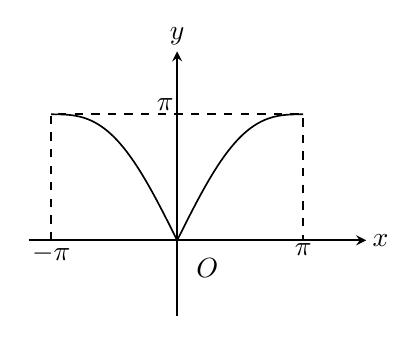
\begin{tikzpicture}[x=1.6cm,y=1.6cm,line width=.6pt,>=stealth,font=\normalsize]
\coordinate (O) at (0,0);
\coordinate (Xl) at (-1.18,0);
\coordinate (Xr) at (1.5,0);
\coordinate (Yb) at (0,-0.6);
\coordinate (Yt) at (0,1.5);
\coordinate (Xm) at (-1,0);
\coordinate (Xp) at (1,0);
\coordinate (Yp) at (0,1);
\coordinate (Lmt) at (-1,1);
\coordinate (Rpt) at (1,1);
\draw[dashed] (Xm)--(Lmt)--(Rpt)--(Xp);
\draw[->] (Xl)--(Xr) node[right=2pt,inner sep=0pt] {$x$};
\draw[->] (Yb)--(Yt) node[above=2pt,inner sep=0pt] {$y$};
\draw[domain=-1:0,samples=121] plot (\x,{abs(\x+sin(deg(pi*\x))/pi)});
\draw[domain=0:1,samples=121] plot (\x,{abs(\x+sin(deg(pi*\x))/pi)});
\node[inner sep=0pt] at (0.24,-0.22) {$O$};
\node[below=1pt,inner sep=0pt] at (Xm) {$-\pi$};
\node[below=1pt,inner sep=0pt] at (Xp) {$\pi$};
\node[above left=1pt,inner sep=0pt] at (Yp) {$\pi$};
\end{tikzpicture}
